\documentclass[12pt]{article}

\usepackage{fullpage}
\usepackage{float}
\usepackage{multirow}
\usepackage[hidelinks]{hyperref}
\usepackage{graphicx}

\title{CSD316 - Assignment 2}
\author{Pranav Dahiya}
\date{1710110249}

\begin{document}

\maketitle

\subsection*{Question 1}

data\_generation.py generates 1000 data points randomly following the specifications given in the question with $a = 1$ and $m$ is 5, 10 and 20. This was done 3 times in order to validate results. The data can be found in folders data\_1 to data\_3. The results for each subpart are given in this file whereas the weights for each dataset are in csv files in their respective folders.\\

The results for the batch and increment algorithm are in tables \ref{tab:batch_and_increment_const} and \ref{tab:batch_and_increment_variable}. The constant learning rate used was $\rho = 3 * 10^{-6}$ whereas the variable learning rate was $\rho(i)=\frac{1.25}{1000+i}$.

\begin{table}[H]
  \centering
  \caption{Batch and Increment with Constant Learning Rate}
  \label{tab:batch_and_increment_const}
  \begin{tabular}{c|c|c}
    Dataset & No of separating dimensions & Iterations \\
    \hline
    \multirow{3}{*}{1} & 5 & 99\\
    & 10 & 91\\
    & 20 & 102\\
    \hline
    \multirow{3}{*}{2} & 5 & 170\\
    & 10 & 72\\
    & 20 & 56\\
    \hline
    \multirow{3}{*}{3} & 5 & 142\\
    & 10 & 114\\
    & 20 & 40\\
  \end{tabular}
\end{table}

\begin{table}[H]
  \centering
  \caption{Batch and Increment with Variable Learning Rate}
  \label{tab:batch_and_increment_variable}
  \begin{tabular}{c|c|c}
    Dataset & No of separating dimensions & Iterations \\
    \hline
    \multirow{3}{*}{1} & 5 & 121\\
    & 10 & 191\\
    & 20 & 41\\
    \hline
    \multirow{3}{*}{2} & 5 & 99\\
    & 10 & 94\\
    & 20 & 32\\
    \hline
    \multirow{3}{*}{3} & 5 & 272\\
    & 10 & 70\\
    & 20 & 59\\
  \end{tabular}
\end{table}

The datasets were made nonseparable by generating 50 more points for each dataset according to the given specifications. The python script for the same is nonseparable\_data\_generation.py. The pocket algorithm is implemented in pocket.py. The results for the pocket algorithm are given below in table \ref{tab:pocket}. Each perceptron is trained for 500 iterations.

\begin{table}[H]
  \centering
  \caption{Pocket Algorithm}
  \label{tab:pocket}
  \begin{tabular}{c|c|c}
    Dataset & No of separating dimensions & No of misclassifications \\
    \hline
    \multirow{3}{*}{1} & 5 & 86\\
    & 10 & 92\\
    & 20 & 103\\
    \hline
    \multirow{3}{*}{2} & 5 & 88\\
    & 10 & 102\\
    & 20 & 98\\
    \hline
    \multirow{3}{*}{3} & 5 & 83\\
    & 10 & 82\\
    & 20 & 99\\
  \end{tabular}
\end{table}

The least mean square algorithm script is in least\_mean\_square.py. The results are given below in table \ref{tab:least_mean_square}.

\begin{table}[H]
  \centering
  \caption{Least Mean Square Algorithm}
  \label{tab:least_mean_square}
  \begin{tabular}{c|c|c}
    Dataset & No of separating dimensions & No of misclassifications \\
    \hline
    \multirow{3}{*}{1} & 5 & 109\\
    & 10 & 157\\
    & 20 & 132\\
    \hline
    \multirow{3}{*}{2} & 5 & 86\\
    & 10 & 123\\
    & 20 & 122\\
    \hline
    \multirow{3}{*}{3} & 5 & 106\\
    & 10 & 117\\
    & 20 & 127\\
  \end{tabular}
\end{table}

Figure \ref{fig:separating_dimensions} shows the number of iterations taken to reach convergence for the batch and increment algorithm on the separable dataset as the number of separating dimensions increases. The general trend is that the iterations to convergence decrease as the number of separating dimensions increases.

\begin{figure}[H]
  \centering
  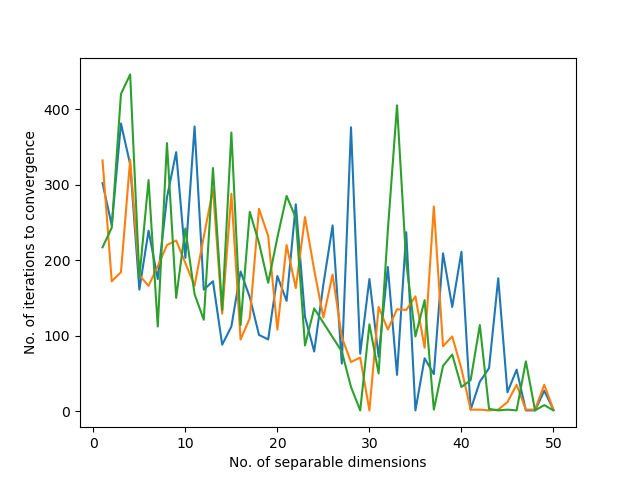
\includegraphics[width=0.8\textwidth]{Figure_1.png}
  \caption{No. of iterations vs No. of separating dimensions}
  \label{fig:separating_dimensions}
\end{figure}

\newpage

\subsection*{Question 2}

First the entire dataset was was split into training and testing sets using train\_test\_split.py such that 90\% of the entire dataset was randomly chosen for the training set and the rest was the testing set. The vocabulary after stop word removal, lemmatization and thresholding was generated using vocabulary.py. The thresholds of the vocabulary were tuned again for training the preceptron. The lower bound was set to 22 occurrences in the dataset and no upper bound was set to 1290. When choosing an appropriate threshold, a higher accuracy on both the train and test sets was preferred. Then 6 linear classifiers were trained using the least mean square algorithm (spam\_filter\_weights\_1.pickle - spam\_filter\_weights\_12.pickle). The python code for the same can be found in spam\_filter.py. The results are shown in table \ref{tab:spam_filter}. A comparison of the mean performance of the linear classifier vs the naive Bayes classifier are shown in table \ref{tab:spam_filter_comparison}.

\begin{table}[H]
  \centering
  \label{tab:spam_filter}
  \caption{Performance of the linear classifier on lingspam}
  \begin{tabular}{r|c|c|c|c|c}
  & \textbf{TP} & \textbf{FP} & \textbf{TN} & \textbf{FN} \\
  \hline
  1&44&8&232&6\\
  2&42&7&233&8\\
  3&43&4&236&7\\
  4&46&12&228&4\\
  5&45&10&230&5\\
  6&46&12&228&4\\
  \hline
  average=&13.58&25.25&214.75&36.42\\
  \hline
  stadard deviation=&5.63&12.75&12.75&5.63
  \end{tabular}
\end{table}

\begin{table}[H]
  \centering
  \label{tab:spam_filter_comparison}
  \caption{Comparison of Performance of LMS and Naive Bayes on the lingspam dataset}
  \begin{tabular}{r||cc|cc}
    \textbf{Performance Metric} & \multicolumn{2}{|c|}{\textbf{LMS}} & \multicolumn{2}{c}{\textbf{Naive Bayes}} \\
    \hline
    & Mean & $\sigma$ & Mean & $\sigma$ \\
    \hline
    TPR(Recall)&0.89&0.03&0.45&0.10\\
    FPR&0.04&0.01&0.00&0.00\\
    TNR&0.96&0.01&1.00&0.00\\
    Precision&0.84&0.05&0.98&0.03\\
    Accuracy&0.95&0.01&0.91&0.02\\
    F1&0.86&0.01&0.61&0.09\\
  \end{tabular}
\end{table}

The performance of the linear classifier is better than the naive Bayes classifier with regards to TPR, Accuracy and F1 score. However, naive Bayes was better in terms of FPR, TNR and Precision.

\end{document}
